\documentclass{article}
\usepackage{preamble}

\title{Unit 10: The Moon}
\author{Astronomy\footnote{Access for free at \href{\openstax}{\openstax}} \hspace{0.1ex} at Cypress Springs High School}
\date{Updated on \today}

\numberwithin{equation}{section}
\setcounter{section}{10}
\numberwithin{figure}{section}

\usepackage{fancyhdr}
\pagestyle{fancy}
\renewcommand{\headrulewidth}{0pt}
\renewcommand{\headruleskip}{0mm}
\fancyfoot[C]{Access for free at \href{\openstax}{\openstax} \hfill \thepage}
\fancyhead{}

\makenoidxglossaries

\begin{document}

\maketitle

\subsection{General Properties of the Moon} \label{Lg4zN5}


The Moon has only one-eightieth the mass of Earth and about one-sixth Earth's surface gravity---too low to retain an atmosphere. Moving molecules of a gas can escape from a planet just the way a rocket does, and the lower the gravity, the easier it is for the gas to leak away into space. While the Moon can acquire a temporary atmosphere from impacting comets, this atmosphere is quickly lost by freezing onto the surface or by escape to surrounding space. The Moon today is dramatically deficient in a wide range of volatiles, those elements and compounds that evaporate at relatively low temperatures. Some of the Moon's properties are summarized in the table below, along with comparative values for Mercury.

\vspace{1em}

\begin{minipage}{0.35\textwidth}
    \centering
    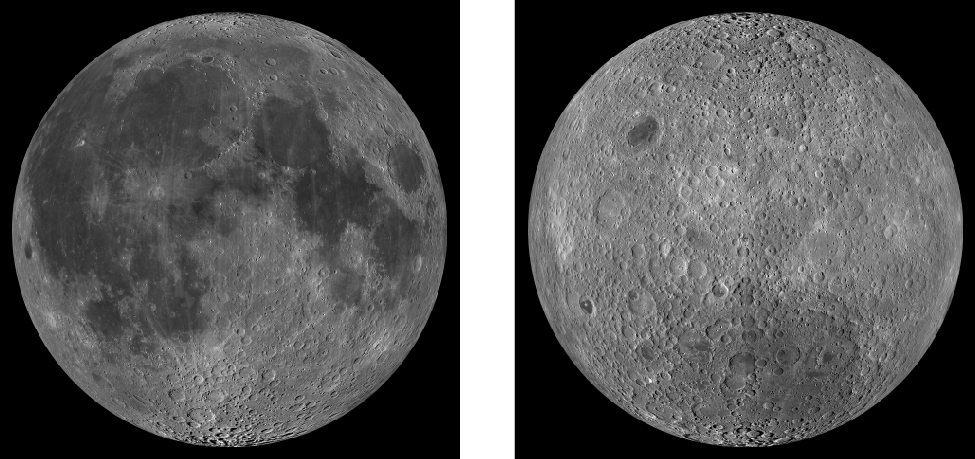
\includegraphics[width=4cm,trim={0cm 0cm 8cm 0cm}, clip]{Figure9.2.jpg}
\end{minipage}%
\hspace{5mm}%
\begin{minipage}{0.55\textwidth}
    \centering
\begin{tabular}{|c|c|c|}
    \hline
    \textbf{Property} & \textbf{Moon} & \textbf{Mercury} \\
    \hline
    Mass (Earth = 1) & 0.0123 &	0.055\\
    \hline
    Diameter (km) & 3476 & 4878\\
    \hline
    Density (\qty{}{g/cm^3})	& 3.3 & 5.4\\
    \hline
    Surface gravity (Earth = 1)	& 0.17 & 0.38\\
    \hline
    Escape velocity (km/s) & 2.4	& 4.3\\
    \hline
    Rotation period (days)	& 27.3 & 58.65\\
    \hline
    Surface area (Earth = 1) & 0.27	& 0.38\\
    \hline
\end{tabular}
\end{minipage}%




\subsubsection*{Exploration of the Moon}
Most of what we know about the Moon today derives from the US Apollo program, which sent nine piloted spacecraft to our satellite between 1968 and 1972, landing 12 astronauts on its surface. Before the era of spacecraft studies, astronomers had mapped the side of the Moon that faces Earth with telescopic resolution of about 1 kilometer, but lunar geology hardly existed as a scientific subject. All that changed beginning in the early 1960s. Initially, Russia took the lead in lunar exploration with Luna 3, which returned the first photos of the lunar far side in 1959, and then with Luna 9, which landed on the surface in 1966 and transmitted pictures and other data to Earth. However, these efforts were overshadowed on July 20, 1969, when the first American astronaut set foot on the Moon.

\vspace{1em}

The table below summarizes the nine Apollo flights: six that landed and three others that circled the Moon but did not land. The initial landings were on flat plains selected for safety reasons. But with increasing experience and confidence, NASA targeted the last three missions to more geologically interesting locales. The level of scientific exploration also increased with each mission, as the astronauts spent longer times on the Moon and carried more elaborate equipment. Finally, on the last Apollo landing, NASA included one scientist, geologist Jack Schmitt, among the astronauts.

\vspace{1em}

\begin{tabular}{|c|c|c|m{7.7cm}|}
    \hline
    \textbf{Flight} & \textbf{Date} & \textbf{Landing Site} & \textbf{Main Accomplishment} \\
    \hline
    Apollo 8 & Dec. 1968 & -- & First humans to fly around the Moon \\
    \hline
    Apollo 10 & May 1969 & -- & First spacecraft rendezvous in lunar orbit\\
    \hline
    Apollo 11 & July 1969 & Mare Tranquillitatis & First human landing on the Moon; 22 kilograms of samples returned\\
    \hline
    Apollo 12 & Nov. 1969 & Oceanus Procellarum	& First Apollo Lunar Surface Experiment Package (ALSEP); visit to Surveyor 3 lander\\
    \hline
    Apollo 13 & Apr. 1970 &	-- & Landing aborted due to explosion in service module\\
    \hline
    Apollo 14 & Jan. 1971 & Mare Nubium	& First ``rickshaw'' on the Moon\\
    \hline
    Apollo 15 & July 1971 & Mare Imbrium/Hadley & First ``rover;'' visit to Hadley Rille; astronauts traveled 24 kilometers\\
    \hline
    Apollo 16 & Apr. 1972 & Descartes & First landing in highlands; 95 kilograms of samples returned\\
    \hline
    Apollo 17 & Dec. 1972 & Taurus-Littrow highlands & Geologist among the crew; 111 kilograms of samples returned\\
    \hline
\end{tabular}

\vspace{1em}

In addition to landing on the lunar surface and studying it at close range, the Apollo missions accomplished three objectives of major importance for lunar science. First, the astronauts collected nearly 400 kilograms of samples for detailed laboratory analysis on Earth (Figure 9.4). These samples have revealed as much about the Moon and its history as all other lunar studies combined. Second, each Apollo landing after the first one deployed an Apollo Lunar Surface Experiment Package (ALSEP), which continued to operate for years after the astronauts departed. Third, the orbiting Apollo command modules carried a wide range of instruments to photograph and analyze the lunar surface from above.

\vspace{1em}

The last human left the Moon in December 1972, just a little more than three years after Neil Armstrong took his ``giant leap for mankind.'' The program of lunar exploration was cut off mid-stride due to political and economic pressures. It had cost just about \$100 per American, spread over 10 years---the equivalent of one large pizza per person per year. Yet for many people, the Moon landings were one of the central events in twentieth-century history.


\subsection*{\ref{Lg4zN5} Exercises (Part I)}

\begin{exercise}
Why does the Moon lack an atmosphere?
\end{exercise}

\begin{exercise}
    If you could represent the total mass of Earth with the number 1, then what would be the mass of the Moon?
\end{exercise}

\begin{exercise}
    If you could represent the surface gravity on Earth with the number 1, then what would be the surface gravity on the Moon?
\end{exercise}

\begin{exercise}
    What is the Moon's radius (the distance from its surface to its core)?
\end{exercise}

\begin{exercise}
    The Apollo programs are the only ones who have placed humans on the Moon. During the 5 years of activity of this program, how many total humans landed on the Moon?
\end{exercise}

\begin{exercise}
    Which country was the first to send a probe to take photos of the dark side of the Moon?
\end{exercise}

\begin{exercise}
    Name the first (uncrewed) spacecraft that ever landed on the Moon.
\end{exercise}

\begin{exercise}
    Which Apollo mission was the first to land astronauts on the Moon? What was the date on which this milestone in human progress occurred?
\end{exercise}

\begin{exercise}
    List at least one of the three major objectives accomplished by the Apollo missions.
\end{exercise}

\begin{exercise}
    Pick one of the landing sites from the table above. Google-search the landing site, and draw a quick sketch of the approximate location of the site on the surface of the Moon.
\end{exercise}

\clearpage

\subsection{The Lunar Surface} \label{6VsXZc}
\subsubsection*{General Appearance}

If you look at the Moon through a telescope, you can see that it is covered by impact craters of all sizes. The most conspicuous of the Moon's surface features---those that can be seen with the unaided eye and that make up the feature often called ``the man in the Moon''---are vast splotches of darker lava flows.

\vspace{1em}

Centuries ago, early lunar observers thought that the Moon had continents and oceans and that it was a possible abode of life. They called the dark areas ``seas'' (\textit{maria} in Latin, or \textit{mare} in the singular, pronounced ``mah ray''). Their names, Mare Nubium (Sea of Clouds), Mare Tranquillitatis (Sea of Tranquility), and so on, are still in use today. In contrast, the ``land'' areas between the seas are not named. Thousands of individual craters have been named, however, mostly for great scientists and philosophers. Among the most prominent craters are those named for Plato, Copernicus, Tycho, and Kepler. Galileo only has a small crater, however, reflecting his low standing among the Vatican scientists who made some of the first lunar maps.

\vspace{1em}

We know today that the resemblance of lunar features to terrestrial ones is superficial. Even when they look somewhat similar, the origins of lunar features such as craters and mountains are very different from their terrestrial counterparts. The Moon's relative lack of internal activity, together with the absence of air and water, make most of its geological history unlike anything we know on Earth.

\vspace{1em}

\begin{center}
\begin{minipage}{0.45\textwidth}
    \centering
    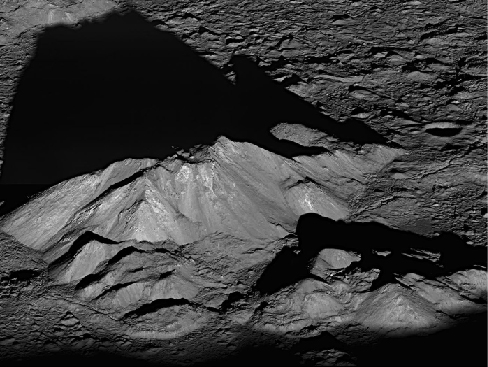
\includegraphics[width=8cm]{Figures/Unit10_Figure9.6.jpeg}
\end{minipage}%
\hspace{5mm}
\begin{minipage}{0.45\textwidth}
    \centering
    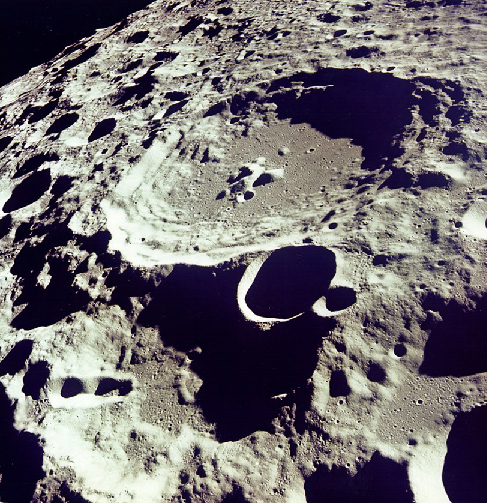
\includegraphics[width=6cm]{Figures/Unit10_Figure9.7.jpeg}
\end{minipage}
\end{center}




\subsection*{\ref{6VsXZc} Exercises}

\begin{exercise}
    What does \textit{mare} mean in Latin? Why were some features on the moon called \textit{maria}?
\end{exercise}

\begin{exercise}
    Name one or more philosophers whom craters on the Moon were named after.
\end{exercise}

\begin{exercise}
    Identify at least one factor that causes the surface features of the Moon and Earth to be vastly different.
\end{exercise}

% \clearpage

% \subsubsection*{Lunar History}

% To trace the detailed history of the Moon or of any planet, we must be able to estimate the ages of individual rocks. Once lunar samples were brought back by the Apollo astronauts, the radioactive dating techniques that had been developed for Earth were applied to them. The solidification ages of the samples ranged from about 3.3 to 4.4 billion years old, substantially older than most of the rocks on Earth. For comparison, as we saw in the chapter on Earth, Moon, and Sky, both Earth and the Moon were formed between 4.5 and 4.6 billion years ago.




% \clearpage
% \subsection*{Lesson Plans}

% \begin{tabular}{|m{0.25\textwidth}|m{0.7\textwidth}|}
%     \hline  
%     \cellcolor{black!20}\textbf{Date} &
%     \cellcolor{black!20}\textbf{Tuesday, Mar, 21 2023} \\
%     \hline
%     Learning Intention (TPO) & We will summarize some properties of the Moon and list accomplishments of the Apollo missions using lecture notes. \\
%     \hline
%     Hook/Warm Up/Opening & View today's Astronomy Picture of the Day (\href{https://apod.nasa.gov/apod/ap230321.html}{click here}) and today's Sky at a Glance (\href{https://skyandtelescope.org/astronomy-news/observing-news/this-weeks-sky-at-a-glance-march-17-26/}{click here}).\\
%     \hline
%     Lesson/Learning Activities & Lecture notes: Moon is Earth's closest neighbor. It has low gravity (one-sixth of Earth), therefore no atmosphere. List relative mass and absolute diameter. Using the table above, list the flight, date, and accomplishment of Apollo missions 8, 11, 13, 15, and 17.\\
%     \hline
%     Graded Activities & N/A\\
%     \hline
%     Closure & Watch a \textit{YouTube} video called ``Apollo 11's journey to the moon'' by \texttt{Vox} (\href{https://youtu.be/OCjhCL2iqlQ}{click here}). Answer student questions.\\  
%     \hline
% \end{tabular}


\end{document}